\subsection{Choques Rotacionais}

O segundo experimento consiste em analisar o choque rotacional de um sistema formado por duas peças cilíndricas rotacionando em torno do mesmo eixo de rotação, sem atrito. Em determinado instante de tempo, a peça que está acima (peça 2) é solta e cai sobre a peça que está abaixo (peça 1) no sistema. Então, devido ao atrito entre as superfícies das duas peças, o conjunto passa a girar a uma velocidade angular comum. O sistema pode ser representado com base na figura abaixo:

\begin{figure}[H]
  \centering
  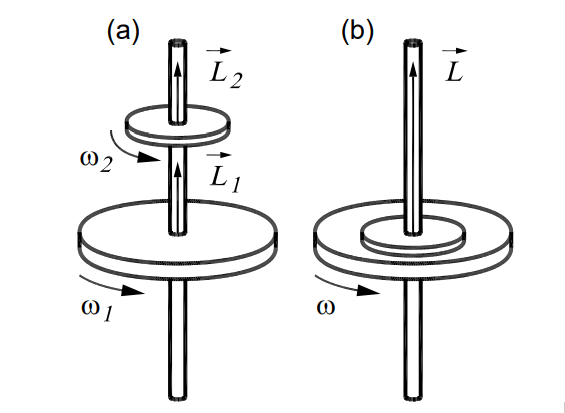
\includegraphics[scale=0.8]{images/choque_rotacional.png}
  \caption{Sistema formado por duas peças cilíndricas que giram em torno do mesmo eixo de rotação com velocidades angulares distintas 1 e 2 (a). Em certo instante de tempo, as peças formam um conjunto que passa a girar a uma mesma velocidade angular (b).}
\end{figure}

Com base na figura anterior, pode-se caracterizar algumas grandezas que foram utilizadas durante o experimento:

\begin{table}[H]
    \centering
    % \begin{tabular}{ |M{2cm}||M{8cm}| }
    \begin{tabular}{ |c||c| }
        \hline
        \textbf{Símbolo} & \textbf{Grandeza}\\
        \hline
        $\omega _1$     & Velocidade Angular inicial da Peça 1\\
        $\omega _2$     & Velocidade Angular inicial da Peça 2\\
        $\omega $       & Velocidade Angular final do conjunto\\
        \hline
        L$_1$   & Momentum Angular inicial da Peça 1\\
        L$_2$   & Momentum Angular inicial da Peça 2\\
        L       & Momentum Angular final do conjunto\\
        \hline
    \end{tabular}
    \caption{Legenda das grandezas}
\end{table}

As peças são caracterizadas como um disco maciço com eixo central (mesmo disco utilizado no experimento anterior com a roda de Maxwell e referido como peça 1) e um cilindro oco (peça 2). Baseado na imagem, também é possível visualizar a direção e sentido dos vetores envolvidos na rotação das peças.\\

Então, inicialmente a peça 1 é colocada em rotação e a peça 2 na parte superior é mantida em repouso e segurada por uma porca (S) para não cair. Ao afrouxar a porca, a peça 2 cai e colide com a peça 1. As velocidades de rotação inicial e final foram medidas com um tacômetro óptico, que conta as franjas na lateral da peça 1.

\begin{figure}[H]
  \centering
  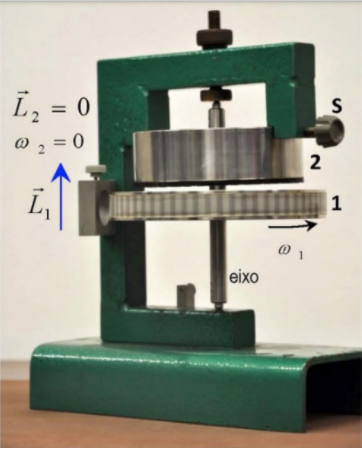
\includegraphics[scale=0.8]{images/experimento_choque.png}
  \caption{Montagem experimental real, com seus respectivos elementos, para analisar o choque rotacional entre duas peças cilíndricas.}
\end{figure}

Com base nas características geométricas e na massa do cilindro oco (Peça 2), foi determinado o Momento de Inércia ($I_2$) com sua respectiva incerteza experimental. As medidas foram determinadas com auxílio de um paquímetro e de uma balança digital para o raio e a massa da peça, respectivamente.\\

Após isso, foi feito uma análise dos resultados representados no segundo vídeo (minuto 31:50 - 36:20) que mostra uma medida quantitativa da diminuição da velocidade angular de rotação da peça 1 devido a torques dissipativos. Com essa análise e o Momento de Inércia da peça 1 ($I_1$) calculado no experimento anterior, foi construído um gráfico da energia de rotação da roda com função do tempo. E então, determinou-se a energia média perdida pelo sistema em um ciclo de oscilação.\\

Para esse experimento, foram realizados três choques rotacionais e em cada um deles foi determinado a velocidade angular imediatamente antes e depois da colisão.Nesse momento, os dados foram obtidos a partir de um software que calcula a velocidade angular com base em um sistema de infravermelho e arduino instalados previamente. O software fornece a velocidade angular em diversos momento e devemos utilizar os pontos que correspondem ao momento imediatamente antes e depois da colisão.\\

Assumindo que houve conservação do momentum angular durante a colisão, determinou-se o Momento de Inércia $I_1$ da peça 1 utilizando a seguinte equação:

\[ \omega = \frac{I_1 \omega_1+I_2 \omega_2}{I_1+I_2} \]

Por fim, calculou-se as energias cinéticas rotacionais, antes e depois da colisão, e sua variação relativa, para, então, verificar se houve ou não conservação da energia cinética. Os resultados obtidos foram comparados ao experimento anterior da Roda de Maxwell para se discutir a confiabilidade de cada método.
